% !TeX program = xelatex
% 编译目录为 docs/，连续运行两次 XeLaTeX 以更新图号与参考文献。
% 初稿由 agy CLI 的 gemini-4-hydrogen-high 撰写，技术表述依据仓库源码与发布版实测记录校订。
\documentclass[a4paper,fontset=fandol,zihao=5]{ctexart}
\usepackage[left=19mm,right=19mm,top=21mm,bottom=19mm,headheight=21pt,headsep=6mm,footskip=9mm]{geometry}
\usepackage{xcolor,graphicx,booktabs,tabularx,array,caption,fancyhdr,microtype}
\usepackage{tikz}
\usetikzlibrary{arrows.meta}
\definecolor{navy}{HTML}{17364A}
\definecolor{teal}{HTML}{126764}
\definecolor{ink}{HTML}{233442}
\definecolor{muted}{HTML}{465D67}
\definecolor{rulegray}{HTML}{B5C7C9}
\definecolor{seaglass}{HTML}{E7F3F0}
\definecolor{cloud}{HTML}{EDF2F4}
\definecolor{sand}{HTML}{FCF3E4}
\definecolor{umber}{HTML}{89551B}
\usepackage[unicode,colorlinks,linkcolor=teal,citecolor=teal,urlcolor=teal]{hyperref}
\hypersetup{pdftitle={基于OpenVLA的无人艇巡检模拟软件开发日志},
  pdfauthor={朱华天，GPT-6.2 Astra，Gemini 4 Hydrogen},
  pdfsubject={港池无人艇中文指令、路径规划、双艇协作与发布验证}}
\urlstyle{tt}
\newcommand{\repolink}[2]{\href{https://github.com/ZHT1235456/OpenVLA-Based-Unmanned-Surface-Vessel-Inspection-Simulator/blob/v1.0.0/#1}{#2}}
\newcommand{\pagetitle}[1]{\section{#1}}
\newcommand{\subhead}[1]{\subsection*{#1}}
\ctexset{section={format=\raggedright\sffamily\bfseries\color{navy}\fontsize{19}{25}\selectfont,
  name={,},number=\arabic{section},aftername=\hspace{.55em},beforeskip=0pt,afterskip=6pt},
  subsection={format=\raggedright\sffamily\bfseries\color{teal}\fontsize{12}{17}\selectfont,
  beforeskip=8pt,afterskip=3pt}}
\setlength{\parindent}{0pt}
\setlength{\parskip}{4.5pt}
\setlength{\tabcolsep}{5pt}
\renewcommand{\arraystretch}{1.22}
\newcolumntype{Y}{>{\raggedright\arraybackslash}X}
\captionsetup[figure]{hypcap=false,font={small},labelfont={bf,color=teal},labelsep=quad,
  justification=raggedright,singlelinecheck=false,skip=4pt}
\pagestyle{fancy}\fancyhf{}
\fancyhead[L]{\small\color{muted}基于OpenVLA的无人艇巡检模拟}
\fancyhead[R]{\small\color{muted}软件开发日志}
\fancyfoot[R]{\small\color{muted}\thepage}
\renewcommand{\headrulewidth}{0.3pt}
\renewcommand{\headrule}{\hbox to\headwidth{\color{rulegray}\leaders\hrule height \headrulewidth\hfill}}
\fancypagestyle{front}{\fancyhf{}\fancyfoot[R]{\small\color{muted}\thepage}\renewcommand{\headrulewidth}{0pt}}
\raggedbottom
\begin{document}
\color{ink}
\thispagestyle{front}
\begin{center}
{\sffamily\bfseries\color{navy}\fontsize{21}{28}\selectfont\mbox{基于OpenVLA的无人艇巡检模拟软件开发日志}\par}
\vspace{4pt}
{\large 朱华天，GPT-6.2 Astra，Gemini 4 Hydrogen\par}
{\color{muted}2026年11月25日\par}
{\fontsize{9}{13}\selectfont\url{https://github.com/ZHT1235456/OpenVLA-Based-Unmanned-Surface-Vessel-Inspection-Simulator}\par}
\end{center}
\vspace{2pt}{\color{rulegray}\hrule height .6pt}\vspace{11pt}

\pagetitle{引言}
在三维港池中，使用者可用中文指令安排一艘或两艘无人艇观察航标、拍照并返回泊位。港池中设有四座巡检航标。木栈桥与防波堤旁各有一座黄标，航道口的红标和绿标组成浮标门。两艘艇共用这张海图，分别从东、西泊位出发。

\begin{minipage}{\linewidth}
\centering
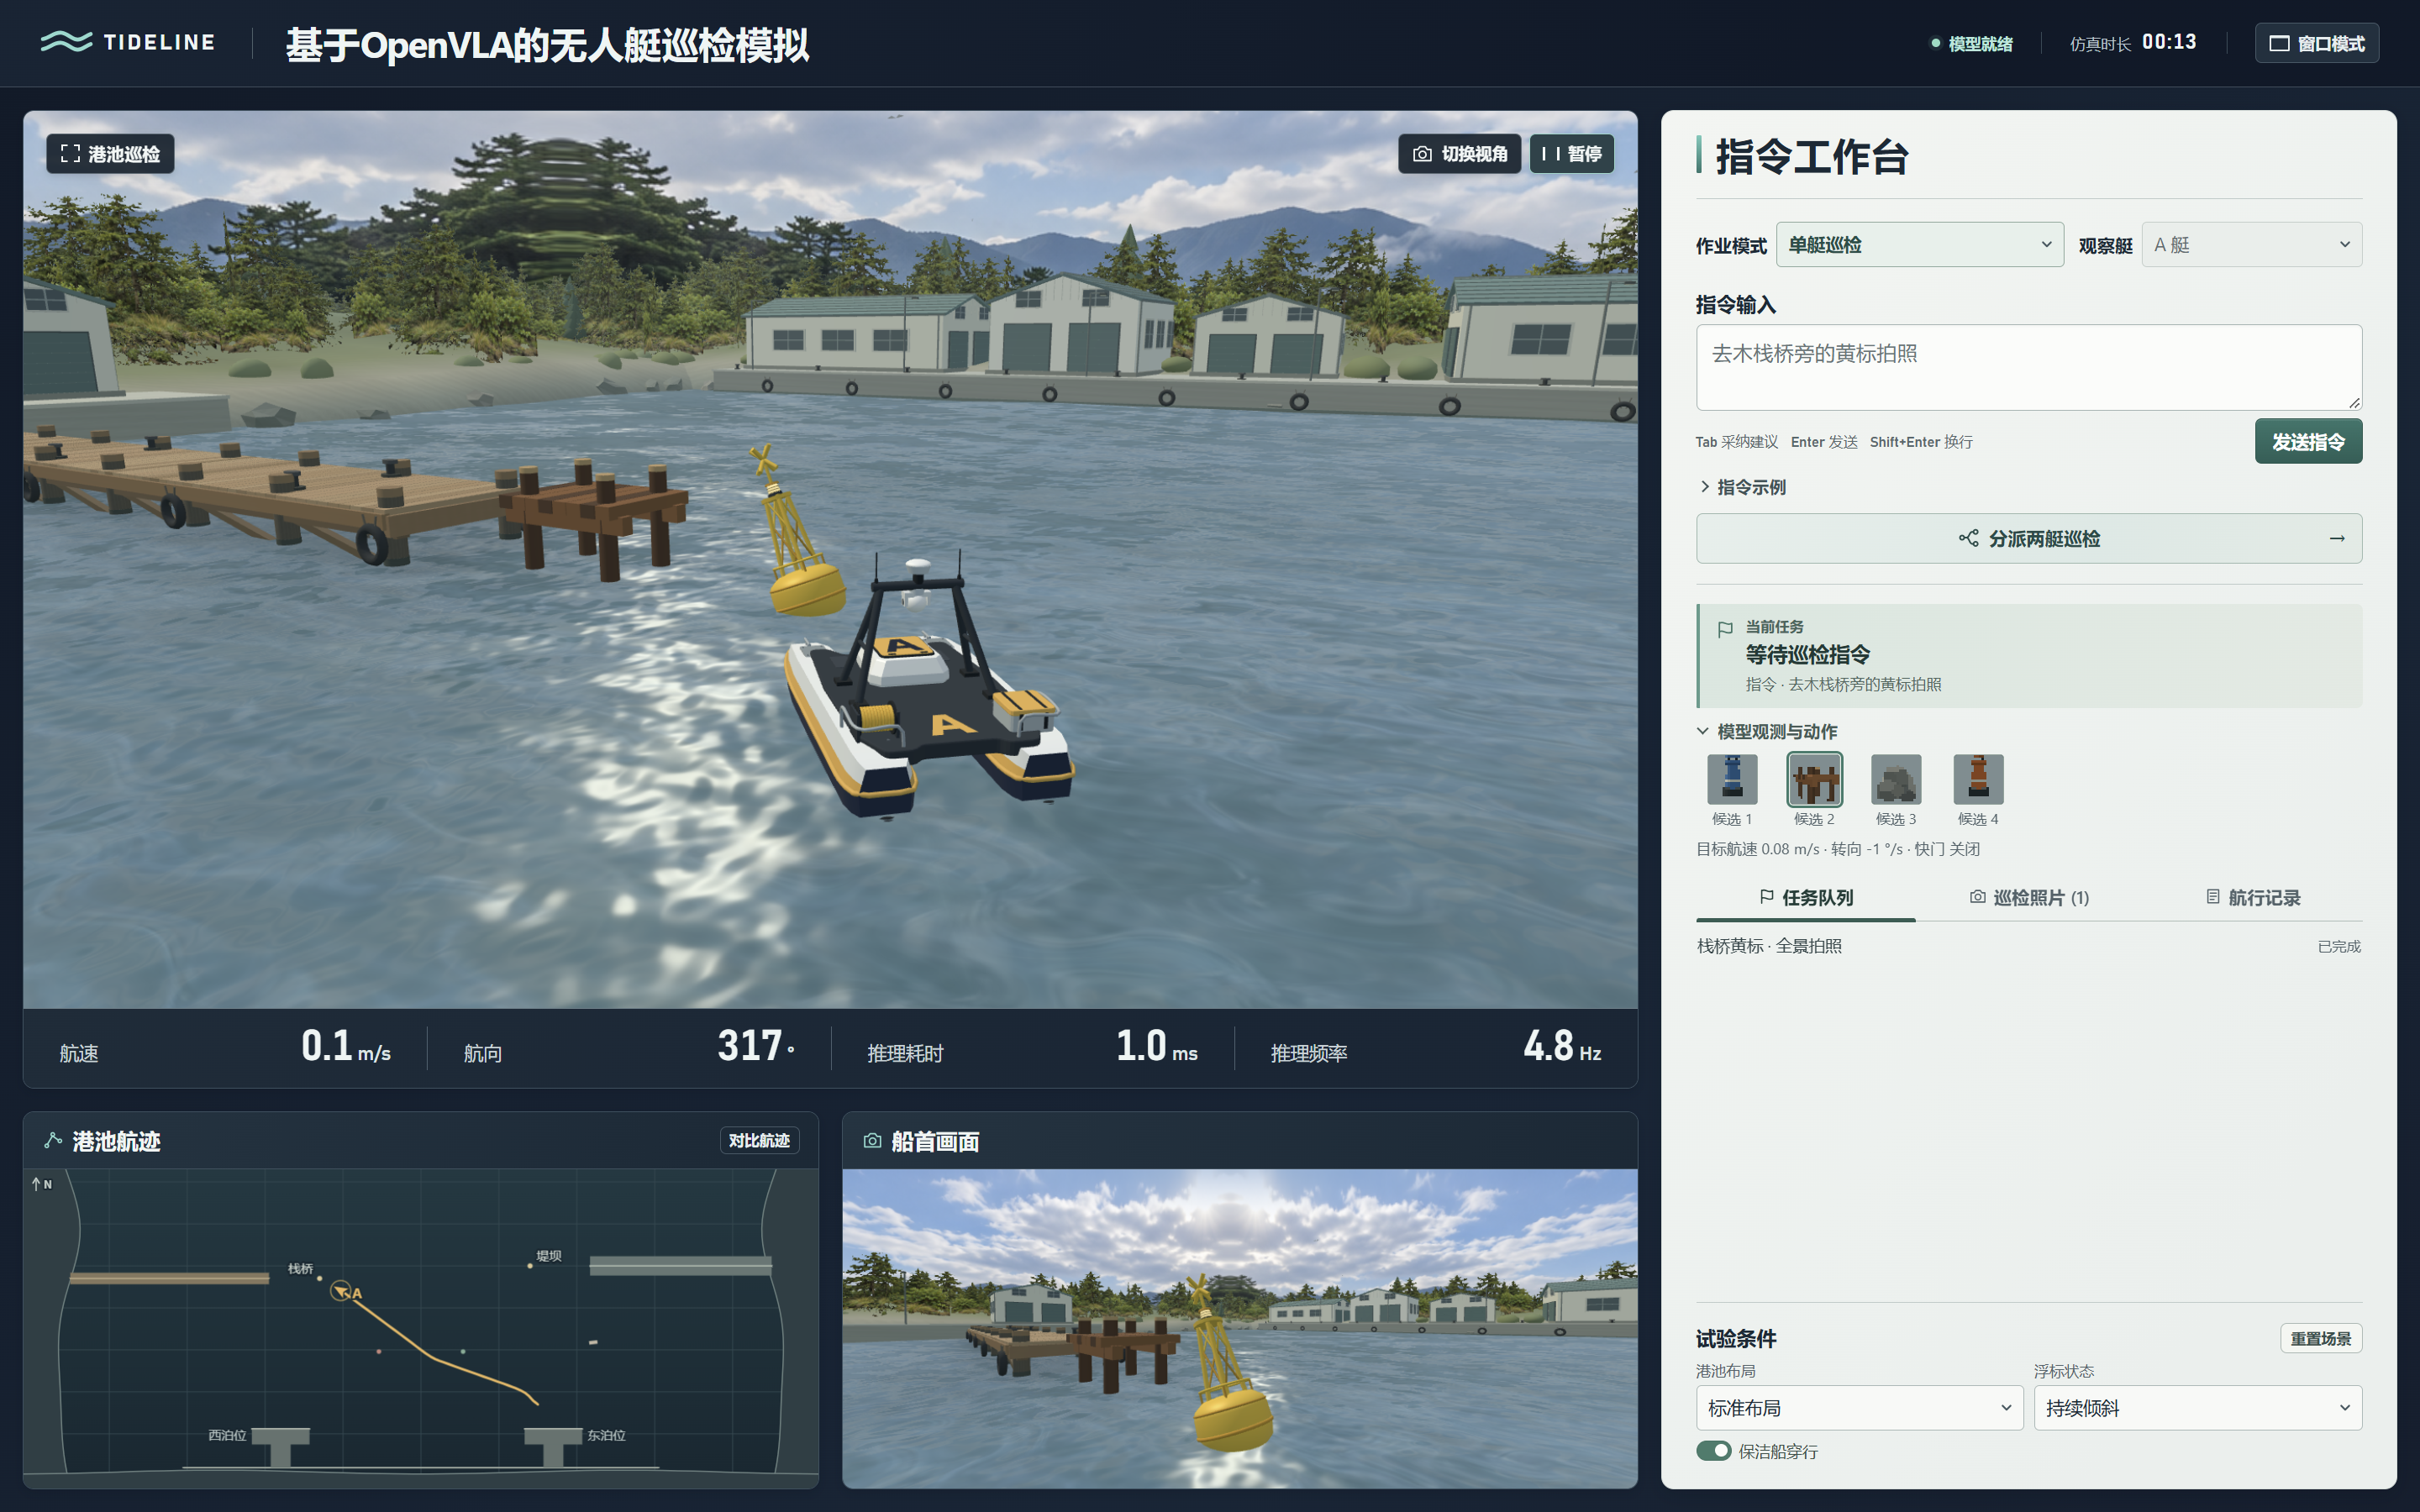
\includegraphics[width=\linewidth]{../verification/desktop.png}
\captionof{figure}{Windows 发布版的单艇巡检。A 艇按指令拍摄木栈桥旁的黄标。下方海图留下驶近目标的航迹，船首画面可用来核对实际入镜的浮标。}\label{fig:desktop}
\end{minipage}

\subhead{在指令工作台安排一次巡检}
以“去浮标门的绿标拍照”为例。在输入框中按 Tab 可填入当前建议并继续修改，按 Enter 发送指令。软件随即核对目标颜色与位置，确认绿标位于浮标门东侧，先规划航线，再抵近拍摄。完成后可在巡检相册查看船首相机拍到的绿标（图~\ref{fig:green}）。

\subhead{观察、拍摄与协作}
输入“先检查红标，再给绿标拍照”，无人艇会先抵近红标观察，再驶向绿标拍一张照片。使用者可以让单艇按序完成，也可以按艇号划分任务。在双艇接力中，先到的艇回传观测方位，另一艘艇据此驶向目标的另一侧补拍。

\newpage
\pagetitle{技术栈与执行流程}
受 OpenVLA 均匀动作离散化方法启发\cite{kim2025openvla}，工程自行训练了港池轻量模型。中文编码器用 UER 两层中文 RoBERTa 初始化，视觉分支取 MobileNetV3-Small 的首层卷积。桌面端实际运行下表中的三个 ONNX 图。

\begin{tabularx}{\linewidth}{@{}>{\bfseries}p{23mm}p{49mm}Y@{}}
\toprule
环节 & 技术与组件 & 在一次巡检中的职责\\
\midrule
训练与导出 & Python、PyTorch、ONNX & 从中文短句、仿真航迹和船首裁片学习指代与动作，在 RTX 4090 上训练后导出。\\
本机推理 & ONNX Runtime Web~\cite{ortweb}、Web Worker、WebAssembly & 后台线程执行 \texttt{language.onnx}、\texttt{navigation.onnx} 和 \texttt{pilot.onnx}。\\
场景与界面 & Three.js、Canvas 2D、Vite & 用 Three.js 绘制港池、艇体和相机画面，用二维海图显示规划航线与已航轨迹。\\
桌面分发 & Tauri 2~\cite{tauri2arch}、Rust、WebView2 & 将网页、模型及运行资源嵌入 Windows 程序，提供全屏与窗口切换。\\
\bottomrule
\end{tabularx}

\subhead{从指令下发到艇上回报}
\begin{minipage}{\linewidth}
\centering
\begin{tikzpicture}[x=1cm,y=1cm,
  main/.style={draw=teal,fill=seaglass,rounded corners=2pt,line width=.55pt,
    text width=5.95cm,minimum height=.98cm,align=center,inner sep=3pt},
  side/.style={draw=rulegray,fill=cloud,rounded corners=2pt,line width=.5pt,
    text width=5.2cm,minimum height=.94cm,align=center,inner sep=3pt},
  stop/.style={side,fill=sand,draw=umber},
  flow/.style={-{Stealth[length=2mm]},draw=teal,line width=.85pt},
  branch/.style={-{Stealth[length=1.7mm]},draw=umber,line width=.65pt},
  hint/.style={font=\scriptsize\sffamily,fill=white,text=muted,inner sep=1.6pt},
  every node/.style={font=\small}]
\node[main] (input) at (0,0) {\textbf{中文指令}\\语言模型判别短句中的目标指代};
\node[main] (assign) at (0,-1.55) {\textbf{校验与派单}\\核对颜色、位置和动作，按艇拆分航段};
\node[main] (route) at (0,-3.1) {\textbf{起航前路径规划}\\从各艇当前位置计算可航路线};
\node[main] (control) at (0,-4.65) {\textbf{实时艇控}\\跟随航路点，预测并避让移动船只};
\node[main] (finish) at (0,-6.2) {\textbf{到站作业}\\按本航段要求观察、拍摄或靠泊};
\node[stop] (conflict) at (8,-1.55) {提示冲突，保留原任务\\可接受建议后重新发送};
\node[stop] (blocked) at (8,-3.1) {停船并显示不可达的任务};
\node[side] (sense) at (8,-4.65) {更新船首裁片、相对几何量和艇位};
\node[side] (report) at (8,-6.2) {记录作业结果，向协作艇回传\\观测方位或已拍照片};
\draw[flow] (input)--(assign);
\draw[flow] (assign)--(route);
\draw[flow] (route)--(control);
\draw[flow] (control)--(finish);
\draw[branch] (assign)--node[hint,above]{矛盾}(conflict);
\draw[branch] (route)--node[hint,above]{无解}(blocked);
\draw[flow] ([yshift=3pt]control.east)--node[hint,above]{推进}([yshift=3pt]sense.west);
\draw[flow] ([yshift=-3pt]sense.west)--node[hint,below]{反馈}([yshift=-3pt]control.east);
\draw[flow] (finish)--(report);
\end{tikzpicture}
\captionof{figure}{一条航行指令的执行流程。接力艇收到有效回报后，按回报方位重新计算自己的作业航段。}\label{fig:flow}
\end{minipage}

\subhead{三个推理图怎样分工}
\texttt{language} 预测目标指代。\texttt{navigation} 结合四张 \(20\times20\) RGB 候选裁片、几何量与目标编码，输出关注对象、航速、转向和快门分数。红绿门标由海图确定身份，\texttt{pilot} 沿用训练好的控制权重，以相对几何量驱艇。明确要求拍照的航段还须满足到站姿态、目标身份和快门条件，才会保存 \(720\times405\) 的船首 JPEG。

展开“模型观测与动作”即可对照当前裁片和模型选中的候选。一次常速双艇复验中，A 艇与 B 艇的艇控推理频率分别为 5.3 Hz 和 5.0 Hz。可在\repolink{src/policy-engine.js}{推理代码}中查看两个艇控图各自的输入。

\newpage
\pagetitle{航路规划与双艇接力}
\subhead{让操作者在起航前看到路线}
以“检查木栈桥旁的黄标，最后返回西泊位”为例。派单后，规划器先在静态海图上为艇体预留通行间距。可以直达时采用直线，否则在可视图中用 A* 搜索航路点\cite{hart1968astar}。若任一航段不可达，艇会停下并显示相应任务。航行途中，保洁船与邻艇的移动交由在线让行逻辑处理。

\begin{minipage}{\linewidth}
\centering
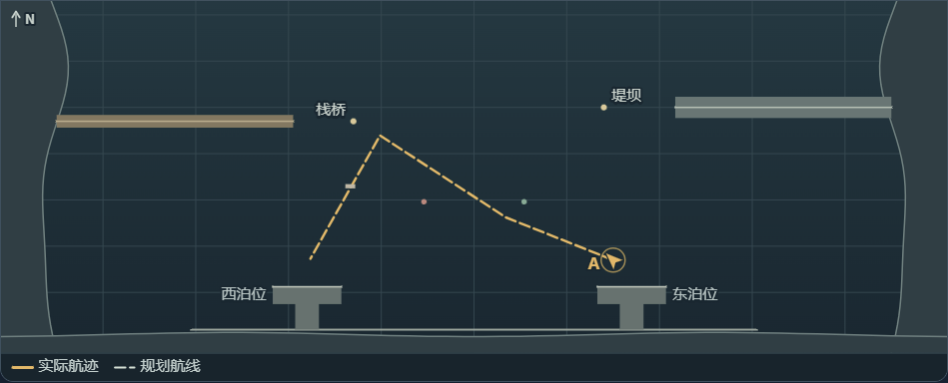
\includegraphics[width=.95\linewidth]{../verification/planned-route.png}
\captionof{figure}{暂停仿真后发送上述指令，A 艇航速仍为 0.0 m/s。琥珀色虚线已连出前往栈桥黄标和返回西泊位的两个航段，规划总长 64.8 m。随后恢复仿真，艇完成观察并停靠西泊位。}\label{fig:route}
\end{minipage}

\subhead{同一目标，两种交接方式}
\begin{minipage}[t]{.55\linewidth}\vspace{0pt}
输入“接力，A 艇只观察栈桥黄标，B 艇收到回报再补拍”时，A 艇先行观察并回传方位。B 艇收到后驶往目标另一侧，整趟任务只有 B 艇拍下的一张照片。接收艇的相册也会显示回传副本，统计拍摄次数时按原始照片计数。

\smallskip
若同时要求 A 艇先拍，首份回报就会附带全景照。图~\ref{fig:relay} 展示了这一版本的交接记录。B 艇相册中可以同时看到 A 艇回传的全景和自己补拍的侧面，艇号和时间能区分两张图片的来源。

\smallskip
两艇每 0.75 仿真秒广播一次艇位，通信模拟的基础单程时延为 0.12 仿真秒。接力艇收到观测回报或照片后才启程复核。
\end{minipage}\hfill
\begin{minipage}[t]{.40\linewidth}\vspace{0pt}
\centering
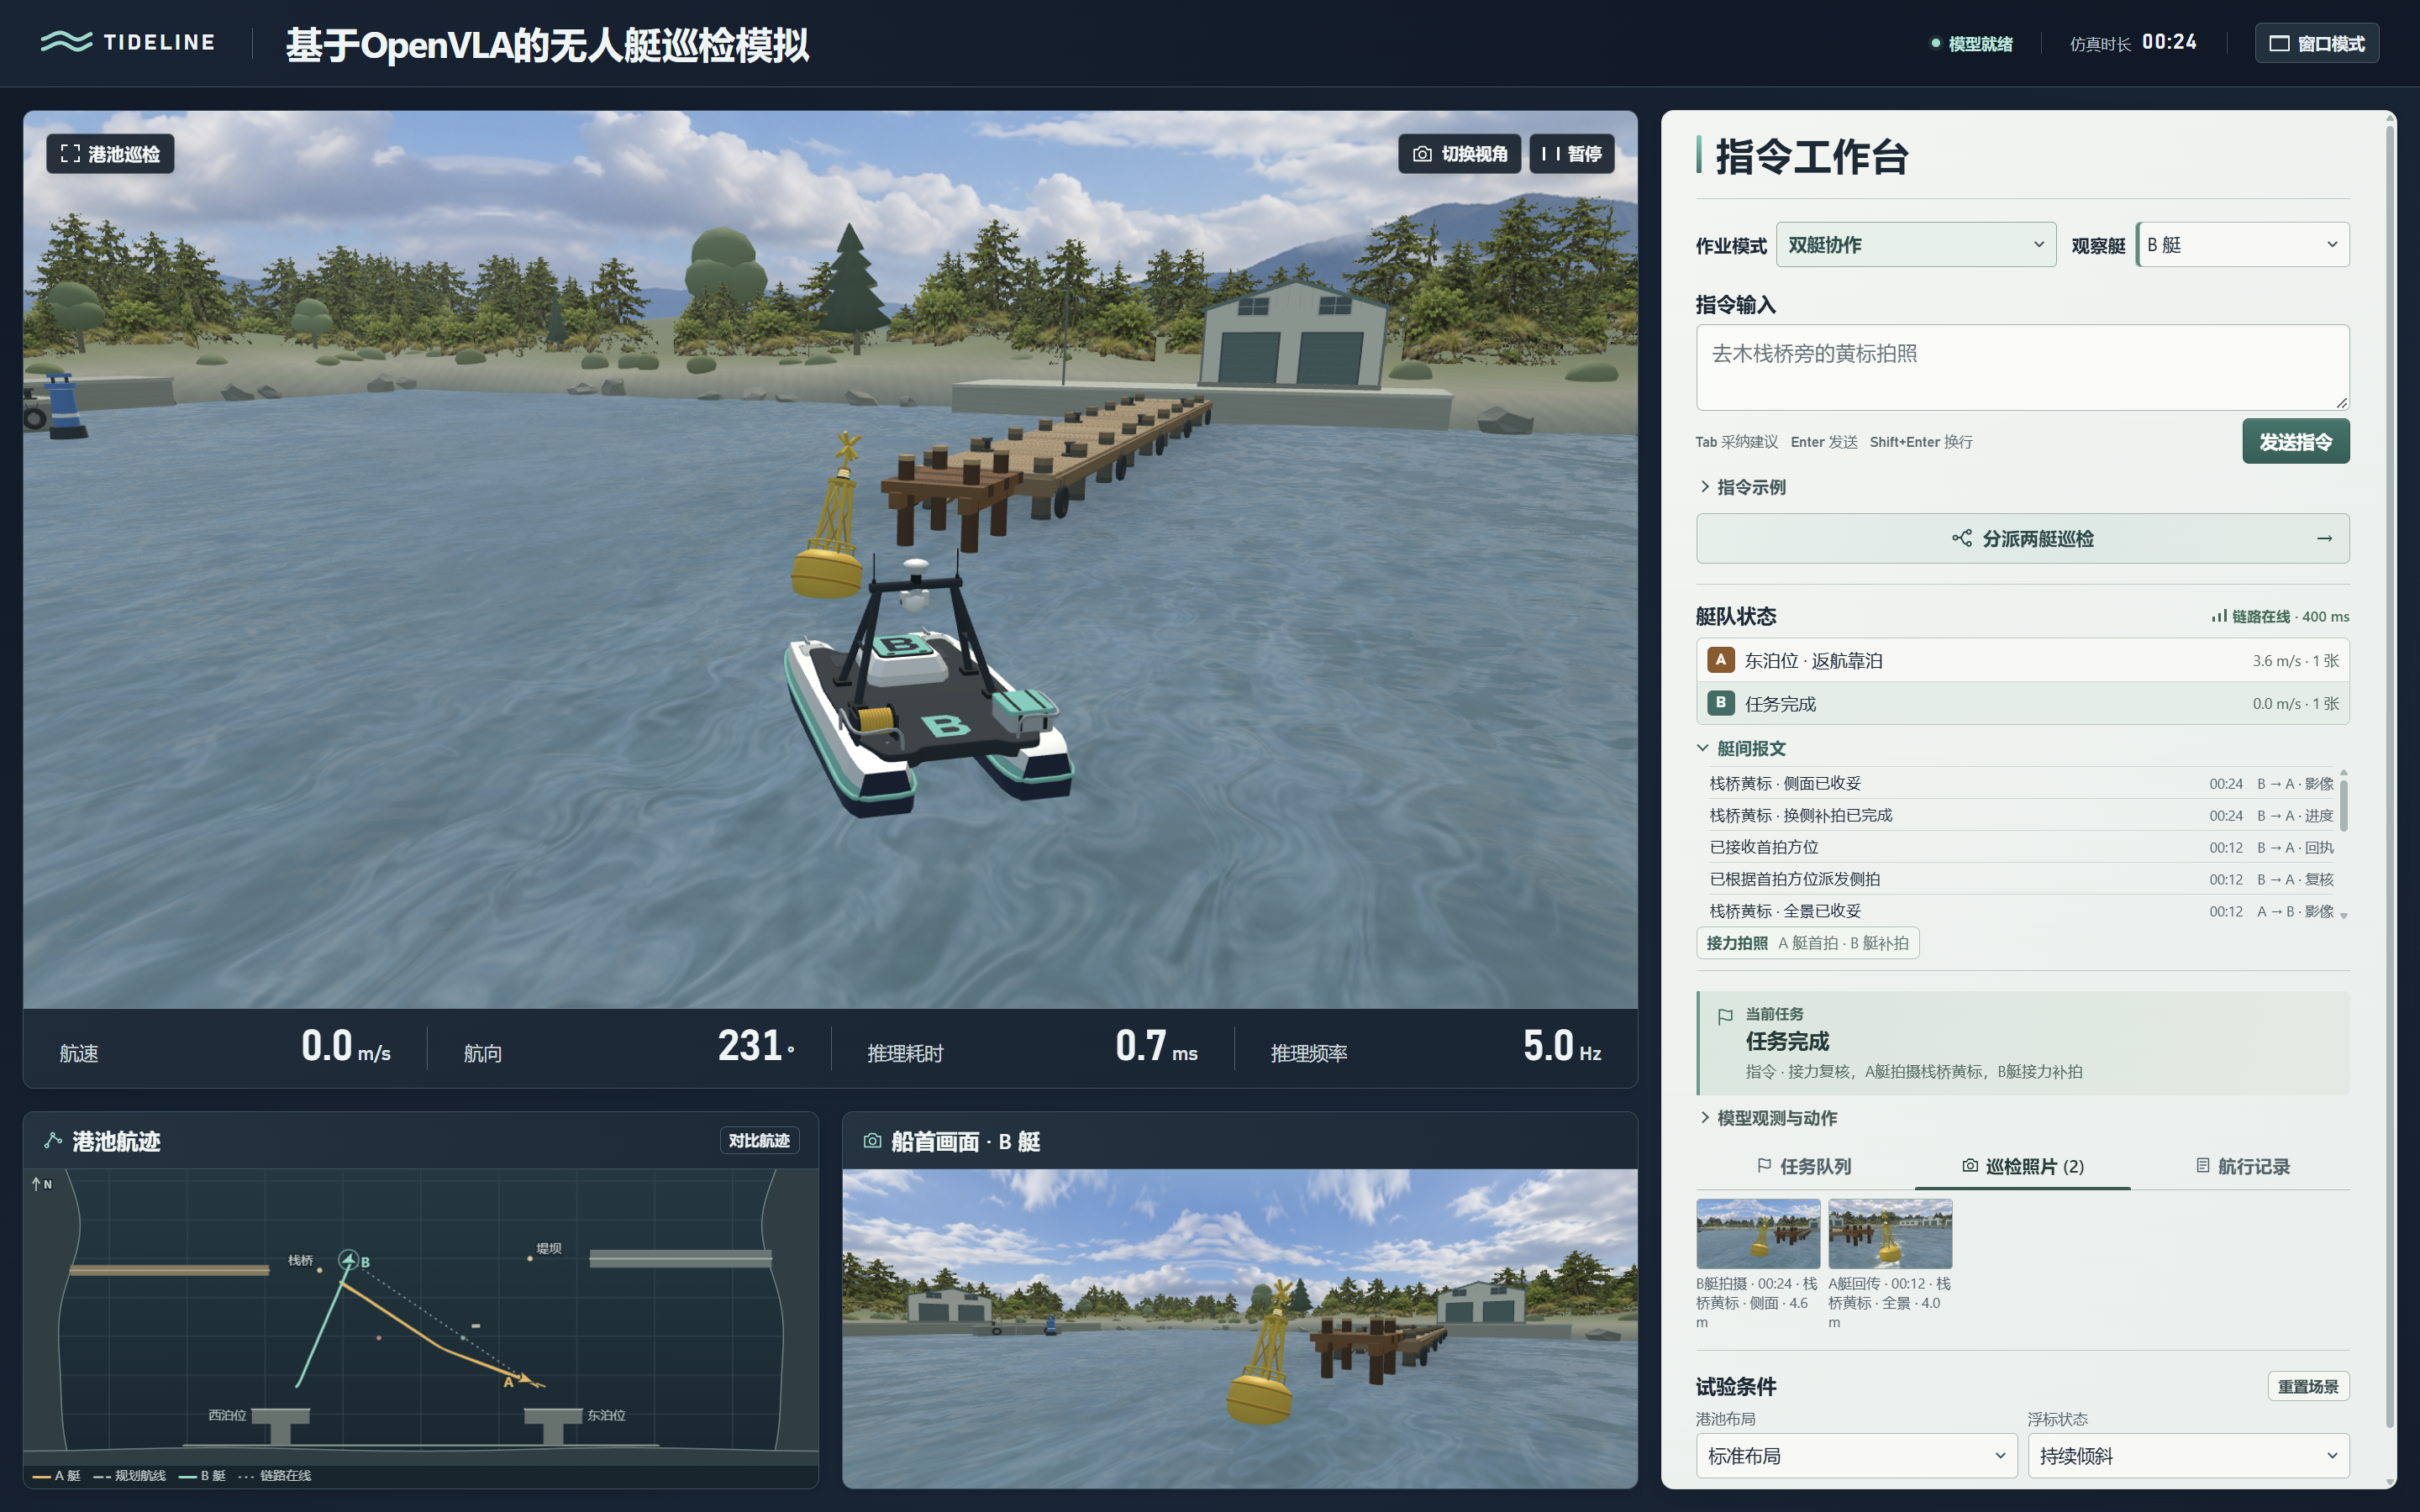
\includegraphics[viewport=1982 205 2848 1107,clip,width=.96\linewidth]{../verification/fleet-handoff.png}
\captionof{figure}{B 艇工作台局部截图。通信记录与两张巡检照片对应同一次接力。}\label{fig:relay}
\end{minipage}

\subhead{途中改变拍摄要求}
单独下发“不要拍照”会撤销待拍航段的快门授权并保留航线。在发布版连续下发“给绿标拍照，最后返回东泊位”“不要拍照”“继续任务”，艇最终停在东泊位，相册新增 0 张。

\newpage
\pagetitle{训练、回归与发布}
\subhead{训练数据与留出结果}
模型训练在实验室 RTX 4090 上使用 PyTorch 2.5.1 完成。艇控策略使用 768 条仿真示范和 70,656 个航行状态，另以不同随机种子生成 96 条验证航迹。中文目标指代模型在 24 条留出短句中正确判别 23 条，具体样本和指标见\repolink{public/models/run.json}{训练记录}。

\subhead{中文指令回放验证}
验证采用 CEGIS 式迭代。先确定每条指令的艇号、目标、动作和预期相册，再从发布版输入框逐条回放，等待 ONNX 推理完成，并核对实际航线、动作与影像。143 条发现集用于调整规则，另有 34 条独立留出指令用于复验。

\begin{tabularx}{\linewidth}{@{}>{\bfseries}p{32mm}p{29mm}Y@{}}
\toprule
核验对象 & 实测结果 & 怎样判定\\
\midrule
发现集与留出集 & 143/143，34/34 & 逐条比对预期结果。两组合计 177 条不同中文指令。\\
执行与拒绝 & 151 条，26 条 & 有效任务核对艇号与动作顺序，预期拒绝项核对拒绝结果。\\
起航前规划 & 164 次 & 按艇核对起航前规划日志、海图航段数和规划距离。\\
实际拍摄 & 83 张 JPEG & 解码实际图像并核对分辨率、目标与取证距离，按场景检查中央颜色。回传副本单独比对。\\
\bottomrule
\end{tabularx}

\vspace{4pt}
\begin{minipage}[c]{.39\linewidth}
\centering
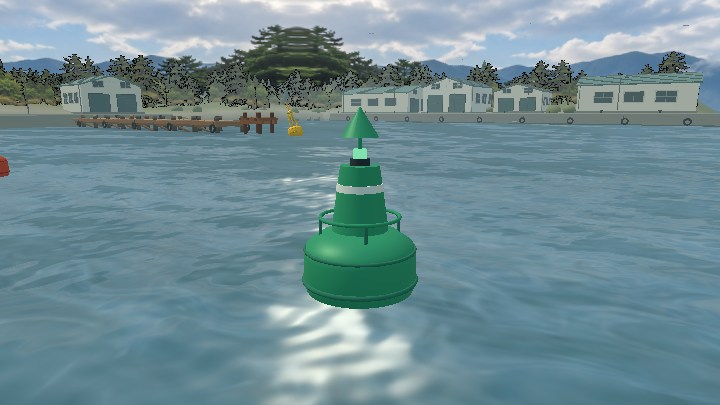
\includegraphics[width=\linewidth]{../verification/gate-green.jpg}
\captionof{figure}{船首相机拍到的浮标门东侧绿标。}\label{fig:green}
\end{minipage}\hfill
\begin{minipage}[c]{.56\linewidth}
\repolink{verification/commands-final.md}{逐条测试报告}列出了输入、派单、照片数和结论。C046 对应单艇观察后返航，C175 对应仅接力艇补拍。

\smallskip
\repolink{verification/desktop.json}{常速桌面复验}还核对了实际入镜的颜色。在图~\ref{fig:green} 中，检测窗口的 18,144 个像素里有 7,216 个绿色像素、0 个黄色像素，和海图登记的绿色门标一致。
\end{minipage}

\subhead{Windows 交付}
v1.0.0 把前端、模型和推理运行资源嵌入单个 Windows x64 EXE，实测为 \textbf{28,124,672 字节（26.82 MiB）}。在具备 Microsoft Edge WebView2 的电脑上，双击即可离线运行。程序默认全屏，右上角可切换为窗口模式。

\begingroup
\small
\setlength{\parskip}{0pt}
\renewcommand{\refname}{参考文献}
\ctexset{section/format=\raggedright\sffamily\bfseries\color{navy}\large,section/beforeskip=8pt,section/afterskip=3pt}
\begin{thebibliography}{4}
\setlength{\itemsep}{2pt}\setlength{\parskip}{0pt}
\bibitem{kim2025openvla} M. J. Kim, K. Pertsch, S. Karamcheti, et al.
\href{https://proceedings.mlr.press/v270/kim25c.html}{OpenVLA: An Open-Source Vision-Language-Action Model}.
CoRL 2024, \emph{Proceedings of Machine Learning Research}, 270, 2679--2713, 2025.
\bibitem{hart1968astar} P. E. Hart, N. J. Nilsson, B. Raphael.
\href{https://doi.org/10.1109/TSSC.1968.300136}{A Formal Basis for the Heuristic Determination of Minimum Cost Paths}.
\emph{IEEE Transactions on Systems Science and Cybernetics}, 4(2), 100--107, 1968.
\bibitem{ortweb} ONNX Runtime. \href{https://onnxruntime.ai/docs/tutorials/web/}{Web tutorials}. 项目官方文档。
\bibitem{tauri2arch} Tauri. \href{https://v2.tauri.app/concept/architecture/}{Tauri Architecture}. 项目官方文档。
\end{thebibliography}
\endgroup
\end{document}
